\documentclass{beamer}
\usepackage{tikz}
\usepackage{xcolor}
\usepackage{amsmath}
\usepackage{amssymb}

\usetikzlibrary{arrows,shapes,positioning,fit,calc,mindmap}

\usetheme{Madrid}
\usecolortheme{beaver}

\title{Analogical Reasoning in Ethics and Law}
\subtitle{Understanding Structure, Strength, and Applications}
\author{Brendan Shea, PhD}
\date{Introduction to Logic}

\begin{document}
	
	\begin{frame}
		\titlepage
	\end{frame}
	
	\begin{frame}{Introduction: What is Analogical Reasoning?}
		\begin{itemize}
			\item \textbf{Analogical reasoning} is the process of drawing connections between two different situations based on relevant similarities.
			\item Analogies allow us to use knowledge about familiar cases to understand or make judgments about unfamiliar cases.
			\item Analogical reasoning is pervasive in human cognition and appears across disciplines including ethics, law, science, and everyday problem-solving.
			\item Unlike deductive reasoning, analogical reasoning does not guarantee certainty but provides plausible conclusions.
		\end{itemize}
		
		\begin{alertblock}{Key Insight}
			Analogical reasoning bridges the gap between what we know and what we seek to understand by identifying meaningful patterns across different domains.
		\end{alertblock}
	\end{frame}
	
	\begin{frame}{Analogical Arguments as Inductive Reasoning}
		\begin{itemize}
			\item \textbf{Inductive reasoning} involves drawing probable conclusions based on patterns and evidence rather than logical necessity.
			\item Analogical arguments are a specific type of inductive reasoning where conclusions are based on relevant similarities between cases.
			\item While deductive arguments aim for certainty, analogical arguments aim for plausibility and probability.
			\item The strength of an analogical argument depends on the quality and relevance of similarities, not just their quantity.
		\end{itemize}
		
		\begin{center}
			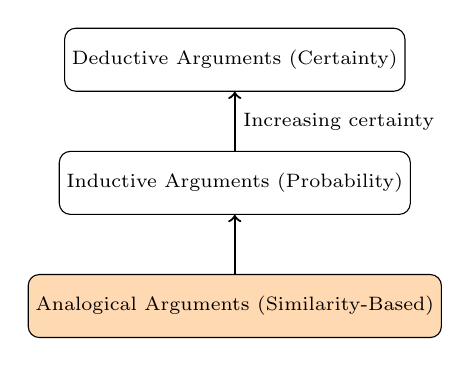
\begin{tikzpicture}[node distance=.75cm]
				\scriptsize
				\node (deductive) [draw, rectangle, rounded corners, minimum width=3cm, minimum height=.8cm] {Deductive Arguments (Certainty)};
				\node (inductive) [draw, rectangle, rounded corners, minimum width=3cm, minimum height=.8cm, below=of deductive] {Inductive Arguments (Probability)};
				\node (analogical) [draw, rectangle, rounded corners, fill=orange!30, minimum width=3cm, minimum height=.8cm, below=of inductive] {Analogical Arguments (Similarity-Based)};
				
				\draw[->, thick] (inductive) -- (deductive) node[midway, right] {Increasing certainty};
				\draw[->, thick] (analogical) -- (inductive) node[midway, right] {};
			\end{tikzpicture}
		\end{center}
	\end{frame}
	
	\begin{frame}{The Basic Structure: Source, Target, and Relevant Similarities}
		\begin{itemize}
			\item Every analogical argument has a \textbf{source domain} (the familiar case about which we have knowledge) and a \textbf{target domain} (the unfamiliar case we're reasoning about).
			\item The argument identifies specific similarities between the source and target domains that are deemed relevant.
			\item Based on these similarities, we infer that what is true in the source domain is likely true in the target domain as well.
			\item The basic form is: "A is to B as C is to D" or "A is like B in relevant ways, B has property P, therefore A likely has property P."
		\end{itemize}
		
		\begin{example}
			\scriptsize
			\textbf{Source:} A parent's responsibility to their child\\
			\textbf{Target:} A government's responsibility to its citizens\\
			\textbf{Similarities:} Power relationship, caretaking role, protection duties\\
			\textbf{Inference:} Like parents, governments have an obligation to ensure basic welfare
		\end{example}
	\end{frame}
	
	\begin{frame}{From Known to Unknown: The Cognitive Leap in Analogies}
		\begin{itemize}
			\item The \textbf{cognitive leap} in analogical reasoning involves transferring knowledge from a well-understood domain to an unfamiliar one.
			\item This process involves recognizing structural patterns rather than merely superficial similarities.
			\item Analogical reasoning allows us to navigate novel ethical and legal situations by connecting them to established precedents or principles.
			\item The cognitive leap is both the strength and potential weakness of analogical reasoning, as it may obscure important differences.
		\end{itemize}
		
		\begin{table}
			\scriptsize
			\begin{tabular}{|p{5cm}|p{5cm}|}
				\hline
				\textbf{Benefits of the Cognitive Leap} & \textbf{Risks of the Cognitive Leap} \\
				\hline
				Enables reasoning about new situations & May overlook critical differences \\
				Builds on established knowledge & Can import irrelevant assumptions \\
				Creates intuitive understanding & May simplify complex issues \\
				Facilitates creative problem-solving & Can lead to false equivalences \\
				\hline
			\end{tabular}
		\end{table}
	\end{frame}
	
	\begin{frame}{The Formula: `A is to B as C is to D'}
		\begin{itemize}
			\item The classic formulation of an analogy follows the pattern \textbf{`A is to B as C is to D'}, creating a proportional relationship.
			\item This structure highlights that it's not just objects that are similar, but the relationships between objects.
			\item In ethical and legal reasoning, we often use this structure to transfer moral or legal principles from established cases to new ones.
			\item Understanding this formula helps us identify when an argument is explicitly or implicitly using analogical reasoning.
		\end{itemize}
		
		\begin{block}{Mathematical Expression}
			If we denote the relation between A and B as R(A,B), the analogical claim is:
			\begin{align}
				R(A,B) \approx R(C,D)
			\end{align}
			Where $\approx$ indicates similarity rather than strict equality.
		\end{block}
	\end{frame}
	
	\begin{frame}{Everyday Analogies: How We Navigate New Situations}
		\begin{itemize}
			\item \textbf{Everyday analogies} are common mental shortcuts we use to understand new situations based on past experiences.
			\item When faced with a new electronic device, we apply knowledge from similar devices we've used before.
			\item In social situations, we often navigate unfamiliar relationships by comparing them to familiar relationship patterns.
			\item Medical decisions frequently rely on analogies to previous health situations we've experienced or learned about.
		\end{itemize}
		
	 \resizebox{0.4\textheight}{!}{%
		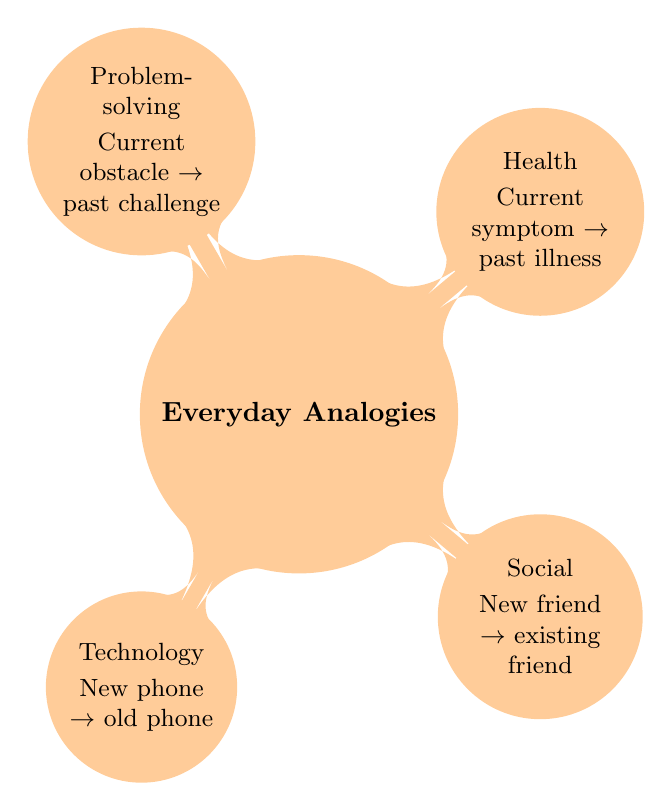
\begin{tikzpicture}[
			mindmap,
			concept color=orange!40,
			text=black,
			grow cyclic,
			level 1/.append style={level distance=4cm, sibling angle=80, font=\small}
			]
			\node[concept, font=\normalsize\bfseries] {Everyday Analogies}
			child { node[concept] {Technology\\[2pt] \small New phone $\to$ old phone} }
			child { node[concept] {Social\\[2pt] \small New friend $\to$ existing friend} }
			child { node[concept] {Health\\[2pt] \small Current symptom $\to$ past illness} }
			child { node[concept] {Problem-solving\\[2pt] \small Current obstacle $\to$ past challenge} };
		\end{tikzpicture}
	}
	\end{frame}
	
	\begin{frame}{Strength Factor: Relevance of Similarities}
		\begin{itemize}
			\item Not all similarities between cases are equally important; the \textbf{relevance} of similarities is crucial to argument strength.
			\item Relevant similarities are those that have a causal or logical connection to the property being projected from source to target.
			\item Irrelevant similarities may be numerous but contribute nothing to the strength of an analogical argument.
			\item Strong analogical arguments focus on structural and functional similarities rather than superficial or coincidental ones.
		\end{itemize}
		
		\begin{exampleblock}{Example: Relevance in Medical Analogies}
			\scriptsize
			A patient with symptoms X, Y, and Z is compared to past patients:
			\begin{itemize}
				\item Patient A: Shares symptoms X, Y, Z and had disease D (relevant similarities)
				\item Patient B: Shares height, hair color, and birth month (irrelevant similarities)
			\end{itemize}
			The analogy to Patient A provides stronger support for diagnosis D despite having the same number of similarities as Patient B.
		\end{exampleblock}
	\end{frame}
	
	\begin{frame}{Strength Factor: Number of Similarities}
		\begin{itemize}
			\item While relevance is primary, the \textbf{number of relevant similarities} does contribute to an analogy's strength.
			\item More points of relevant comparison generally create a stronger inferential bridge between source and target.
			\item The relationship between number of similarities and argument strength is not linear but shows diminishing returns.
			\item A few highly relevant similarities often outweigh many tangentially relevant ones.
		\end{itemize}
		
		\begin{table}
				\scriptsize
			\begin{tabular}{|l|c|c|c|}
				\hline
				\textbf{Analogy Type} & \textbf{Few Similarities} & \textbf{Many Similarities} & \textbf{Determining Factor} \\
				\hline
				Scientific & Potentially Strong & Very Strong & Causal relevance \\
				Legal & Potentially Strong & Strong & Precedent relevance \\
				Moral & Often Weak & Potentially Strong & Principle relevance \\
				Everyday & Usually Weak & Moderately Strong & Practical relevance \\
				\hline
			\end{tabular}
		\end{table}
	\end{frame}
	
	\begin{frame}{Strength Factor: Disanalogies and Counterexamples}
		\begin{itemize}
			\item \textbf{Disanalogies} are relevant differences between the source and target that weaken an analogical argument.
			\item The impact of a disanalogy depends on whether it affects the specific property being projected from source to target.
			\item A single critical disanalogy can undermine an otherwise strong analogical argument with many similarities.
			\item Identifying disanalogies is a key technique for challenging analogical arguments in ethical and legal contexts.
		\end{itemize}
		
		\begin{alertblock}{Warning: Strong Disanalogies}
			When evaluating an analogy, always ask: "Is there a difference between these cases that undermines the very property or principle being transferred from source to target?"
		\end{alertblock}
	\end{frame}
	
	\begin{frame}{Strength Factor: The Base Rate Problem}
		\begin{itemize}
			\scriptsize
			\item The \textbf{base rate problem} refers to how common the projected property is in the general category that includes both source and target.
			\item Analogical arguments are stronger when they project rare or unusual properties rather than common ones.
			\item If a property is common across many cases (high base rate), the specific similarities between source and target become less important.
			\item This factor is often overlooked in everyday analogical reasoning but is crucial in scientific and legal contexts.
		\end{itemize}
		
		\begin{center}
			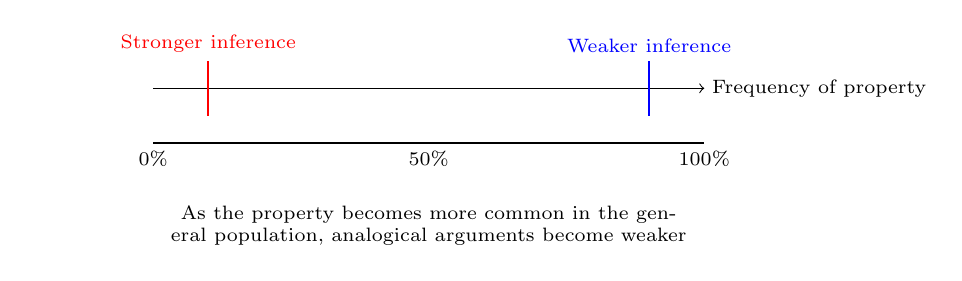
\begin{tikzpicture}[scale = .7]
				\scriptsize
				\draw[thick] (0,0) -- (10,0);
				\node[below] at (0,0) {0\%};
				\node[below] at (10,0) {100\%};
				\node[below] at (5,0) {50\%};
				
				\draw[->] (0,1) -- (10,1) node[right] {Frequency of property};
				
				\draw[thick, red] (1,0.5) -- (1,1.5) node[above] {Stronger inference};
				\draw[thick, blue] (9,0.5) -- (9,1.5) node[above] {Weaker inference};
				
				\node[text width=10cm, align=center] at (5,-1.5) {As the property becomes more common in the general population, analogical arguments become weaker};
			\end{tikzpicture}
		\end{center}
	\end{frame}
	
	\begin{frame}{Evaluating an Analogical Argument: A Step-by-Step Process}
		\begin{itemize}
			\item Step 1: Clearly identify the source domain, target domain, and the property being projected.
			\item Step 2: List all relevant similarities between the source and target, focusing on those related to the projected property.
			\item Step 3: Identify potential disanalogies, especially those that might undermine the projection of the property.
			\item Step 4: Consider the base rate of the property in the general category that includes both source and target.
		\end{itemize}
		
		\begin{exampleblock}{Evaluating Process Example}
			\scriptsize
			\textbf{Argument:} "Artificial intelligence should have legal rights because humans have legal rights, and both can reason and make decisions."
			\begin{enumerate}
				\item \textbf{Source:} Humans; \textbf{Target:} AI; \textbf{Property:} Deserving legal rights
				\item \textbf{Similarities:} Decision-making capacity, reasoning ability
				\item \textbf{Disanalogies:} Consciousness, biological needs, vulnerability, autonomy origin
				\item \textbf{Base rate:} Legal rights are rare among entities in general
			\end{enumerate}
		\end{exampleblock}
	\end{frame}
	
	\begin{frame}{Common Fallacies in Analogical Reasoning}
		\begin{itemize}
			\item The \textbf{False Analogy Fallacy} occurs when an argument relies on similarities that are irrelevant to the conclusion being drawn.
			\item The \textbf{Hasty Generalization} combines weak analogical reasoning with insufficient evidence.
			\item \textbf{Appeal to Tradition} often uses analogies to past practices without considering relevant differences in context.
			\item \textbf{Confirmation Bias} leads us to notice similarities that support our preferred conclusion while ignoring disanalogies.
		\end{itemize}
		
		\begin{block}{Example Fallacies}
			
			\begin{itemize}
				\item \textbf{False Analogy:} "Running a government is just like running a business, so a business leader will be a good president."
				\begin{itemize}
					\scriptsize
					\item Ignores crucial differences in goals (profit vs. public good) and stakeholder relationships
				\end{itemize}
				\item \textbf{Hasty Generalization:} "My friend's diet worked for them, so it will work for everyone."
				\begin{itemize}
					\scriptsize
					\item Overlooks individual biological differences and contexts
				\end{itemize}
			\end{itemize}
		\end{block}
	\end{frame}
	
	
	\begin{frame}{The False Analogy: When Comparisons Mislead}
		\begin{itemize}
			\item A \textbf{false analogy} occurs when the similarities between source and target are superficial or irrelevant to the property being transferred.
			\item False analogies are particularly common in political and moral debates where emotional resonance can mask logical weakness.
			\item The persuasive power of false analogies often stems from their intuitive appeal rather than their logical merit.
			\item Recognizing false analogies requires focusing on whether the similarities genuinely support the conclusion being drawn.
		\end{itemize}
		
		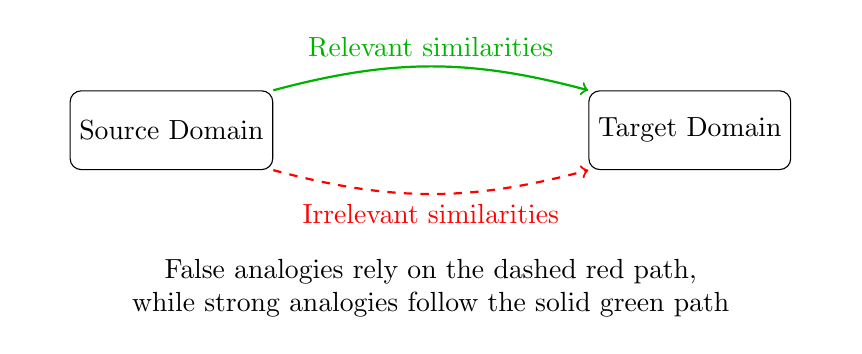
\begin{tikzpicture}[node distance=2cm]
			\node (source) [draw, rectangle, rounded corners, minimum width=2.5cm, minimum height=1cm] {Source Domain};
			\node (target) [draw, rectangle, rounded corners, minimum width=2.5cm, minimum height=1cm, right=4cm of source] {Target Domain};
			
			\draw[->, bend left=15, thick, green!70!black] (source.north east) to node[above, align=center] {Relevant similarities} (target.north west);
			\draw[->, bend right=15, dashed, thick, red] (source.south east) to node[below, align=center] {Irrelevant similarities} (target.south west);
			
			\node[text width=10cm, align=center] at ($(source)!0.5!(target)+(0,-2)$) {False analogies rely on the dashed red path,\\while strong analogies follow the solid green path};
		\end{tikzpicture}
	\end{frame}
	
	\begin{frame}{Competing Analogies in Bioethics: The Abortion Debate}
		\begin{itemize}
			\item The abortion debate features competing analogies that fundamentally shape moral reasoning on both sides.
			\item Each side employs analogies that highlight different aspects of pregnancy and fetal development.
			\item These analogies influence intuitions about the moral status of the fetus and the permissibility of abortion.
			\item Analyzing these analogies reveals how analogical reasoning can frame complex ethical questions.
		\end{itemize}
		
		\begin{alertblock}{The Role of Analogies in Moral Status Questions}
			Analogies are especially powerful in bioethics because they help us apply familiar moral categories to entities with unclear moral status. The strength of these analogies significantly impacts the persuasiveness of each position.
		\end{alertblock}
	\end{frame}
	
	\begin{frame}{Pro-Life Analogies: Fetus as Developing Person}
		\begin{itemize}
			\item Pro-life arguments often employ the \textbf{Child Development Analogy}, comparing a fetus to a newborn, infant, or young child.
			\item This analogy emphasizes the continuity of human development along a single biological trajectory.
			\item The analogy suggests that differences between a fetus and child (size, location, development stage) are morally irrelevant.
			\item Like the "acorn is to oak tree" comparison, this analogy focuses on natural potential and inherent nature.
		\end{itemize}
		
		\begin{table}
			\scriptsize
			\begin{tabular}{|p{3cm}|p{4cm}|p{4cm}|}
				\hline
				\textbf{Analogy Used} & \textbf{Key Similarity} & \textbf{Moral Implication} \\
				\hline
				Fetus as sleeping person & Temporarily inactive but will naturally "awaken" & Killing is wrong despite temporary unconsciousness \\
				\hline
				Fetus as young child & Same entity at different stages & Developmental stage doesn't affect moral worth \\
				\hline
				Fetus as human with disability & Limited current capacities & Capacities don't determine human rights \\
				\hline
			\end{tabular}
		\end{table}
	\end{frame}
	
	\begin{frame}{Pro-Choice Analogies: Fetus as Biological Entity}
		\begin{itemize}
			\scriptsize
			\item Pro-choice arguments often use the \textbf{Organ or Tissue Analogy}, comparing a fetus (especially early-stage) to biological material.
			\item This analogy emphasizes the biological integration with and dependence on the pregnant person's body.
			\item The analogy suggests that, like other body tissues, the fetus lacks independent moral status separate from the person carrying it.
			\item These analogies focus on current capabilities rather than future potential.
		\end{itemize}
		
		\begin{center}
			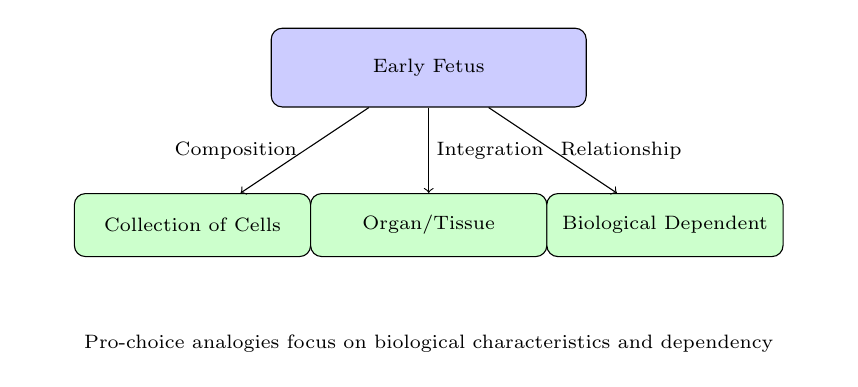
\begin{tikzpicture}
				\scriptsize
				% Pro-choice main concept
				\node[draw, rectangle, rounded corners, fill=blue!20, minimum width=4cm, minimum height=1cm] (main) at (0,0) {Early Fetus};
				
				% Analogies
				\node[draw, rectangle, rounded corners, fill=green!20, minimum width=3cm, minimum height=0.8cm] (cells) at (-3,-2) {Collection of Cells};
				\node[draw, rectangle, rounded corners, fill=green!20, minimum width=3cm, minimum height=0.8cm] (organ) at (0,-2) {Organ/Tissue};
				\node[draw, rectangle, rounded corners, fill=green!20, minimum width=3cm, minimum height=0.8cm] (dependent) at (3,-2) {Biological Dependent};
				
				% Connections
				\draw[->] (main) -- node[left] {Composition} (cells);
				\draw[->] (main) -- node[right] {Integration} (organ);
				\draw[->] (main) -- node[right] {Relationship} (dependent);
				
				% Emphasis on key analogical features
				\node[text width=10cm, align=center] at (0,-3.5) {Pro-choice analogies focus on biological characteristics and dependency};
			\end{tikzpicture}
		\end{center}
	\end{frame}
	
	\begin{frame}{Case Study: Singer's Drowning Child Analogy}
		\begin{itemize}
			\item Peter Singer's \textbf{Drowning Child Analogy} argues that our moral duties to distant strangers are similar to our duties to those nearby.
			\item The source domain involves a child drowning in a shallow pond whom you could save at minor cost (ruined clothes).
			\item Singer argues that distance is not morally relevant, so our duty to save lives through charitable donations is analogous to saving the drowning child.
			\item This analogy challenges the common intuition that we have stronger obligations to those physically near us than to distant strangers.
		\end{itemize}
		
		\begin{block}{Singer's Argument Structure}
			\scriptsize
			\begin{enumerate}
				\item If you can prevent something bad without sacrificing anything of comparable moral importance, you ought to do it.
				\item Death from poverty-related causes is bad.
				\item By donating to effective charities, you can prevent such deaths without sacrificing anything of comparable moral importance.
				\item Therefore, you ought to donate to effective charities.
			\end{enumerate}
		\end{block}
	\end{frame}
	
	\begin{frame}{The Trolley Problem: A Study in Moral Analogies}
		\scriptsize
		\begin{itemize}
			\item The \textbf{Trolley Problem} involves comparing two scenarios to explore moral intuitions about causing harm versus allowing harm.
			\item In the first scenario, diverting a trolley from five people to one seems morally permissible to many.
			\item In the second scenario, pushing a large person off a bridge to stop the trolley seems impermissible to most, despite the same numerical outcome.
			\item The comparison reveals that factors beyond simple utilitarian calculus influence our moral judgments.
		\end{itemize}
		
		\begin{center}
			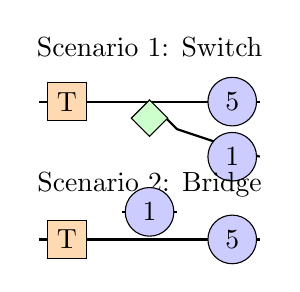
\begin{tikzpicture}[scale = .7]
				% Scenario 1
				\node at (0,2) {Scenario 1: Switch};
				
				% Tracks
				\draw[thick] (-2,1) -- (2,1);
				\draw[thick] (0,1) -- (0.5,0.5) -- (2,0);
				
				% Trolley
				\node[rectangle, draw, fill=orange!30] at (-1.5,1) {T};
				
				% People
				\node[circle, draw, fill=blue!20] at (1.5,1) {5};
				\node[circle, draw, fill=blue!20] at (1.5,0) {1};
				
				% Switch
				\node[diamond, draw, fill=green!20] at (0,0.7) {};
				
				% Scenario 2
				\node at (0,-0.5) {Scenario 2: Bridge};
				
				% Bridge and track
				\draw[thick] (-2,-1.5) -- (2,-1.5);
				\draw[thick] (-0.5,-1) -- (0.5,-1);
				
				% Trolley
				\node[rectangle, draw, fill=orange!30] at (-1.5,-1.5) {T};
				
				% People
				\node[circle, draw, fill=blue!20] at (1.5,-1.5) {5};
				\node[circle, draw, fill=blue!20] at (0,-1) {1};
			\end{tikzpicture}
		\end{center}
	\end{frame}
	
	\begin{frame}{Analogies in Ethics: From Intuition to Principle}
		\begin{itemize}
			\item Ethical analogies often help bridge the gap between moral intuitions about specific cases and general moral principles.
			\item The process of \textbf{reflective equilibrium} involves adjusting both our intuitions about cases and our moral principles until they align.
			\item Strong analogies in ethics reveal morally relevant features that might be obscured in complex real-world situations.
			\item Competing analogies in ethical debates often reflect different underlying moral frameworks (e.g., consequentialist vs. deontological).
		\end{itemize}
		
	\end{frame}
	
	\begin{frame}{Case-Based Reasoning in Law: The Concept of Precedent}
		\begin{itemize}
			\item \textbf{Precedent} is the legal principle that similar cases should be decided similarly, making legal reasoning inherently analogical.
			\item The doctrine of \textbf{stare decisis} ("to stand by decisions") requires judges to respect prior rulings in analogous cases.
			\item Legal analogical reasoning involves identifying relevant similarities between a current case and precedent cases.
			\item Unlike scientific analogies, legal analogies operate within an institutionalized system that formally requires consistency.
		\end{itemize}
		
		\begin{exampleblock}{The Structure of Legal Reasoning By Analogy}
			\scriptsize
			\begin{enumerate}
				\item Case A was decided in a certain way.
				\item Case B resembles Case A in relevant respects.
				\item Therefore, Case B should be decided the same way as Case A.
				\item \textit{Or}: Case B differs from Case A in relevant respects.
				\item Therefore, Case B should be distinguished from Case A and decided differently.
			\end{enumerate}
		\end{exampleblock}
	\end{frame}
	
\begin{frame}{The Role of Disanalogies in Legal Arguments}
	\begin{itemize}
		\item \textbf{Distinguishing} cases is the legal practice of identifying relevant differences that justify different legal treatment.
		\item Effective legal advocacy often involves emphasizing similarities when precedent favors your position and disanalogies when it doesn't.
		\item Courts must determine whether disanalogies are legally significant enough to justify departing from precedent.
		\item The ability to identify meaningful disanalogies allows the law to evolve while maintaining consistency.
	\end{itemize}
	
	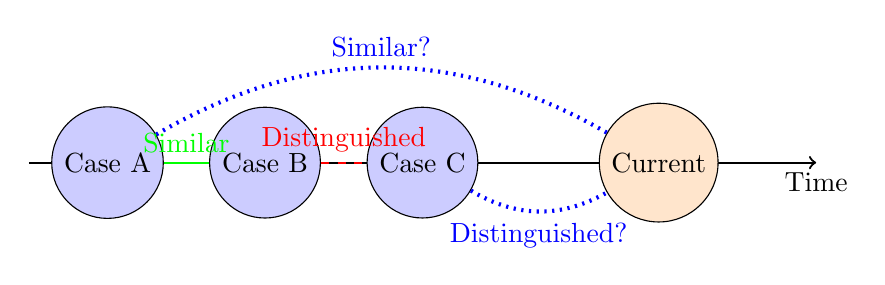
\begin{tikzpicture}
		% Timeline
		\draw[->, thick] (-5,0) -- (5,0);
		\node[below] at (5,0) {Time};
		
		% Precedent cases
		\node[circle, draw, fill=blue!20] (case1) at (-4,0) {Case A};
		\node[circle, draw, fill=blue!20] (case2) at (-2,0) {Case B};
		\node[circle, draw, fill=blue!20] (case3) at (0,0) {Case C};
		
		% Current case
		\node[circle, draw, fill=orange!20] (current) at (3,0) {Current};
		
		% Similarities and differences
		\draw[-, thick, green] (case1) -- node[above] {Similar} (case2);
		\draw[-, thick, red, dashed] (case2) -- node[above] {Distinguished} (case3);
		
		% Question
		\draw[-, thick, blue, dotted, line width=1.5pt] (case1) to[bend left] node[above] {Similar?} (current);
		\draw[-, thick, blue, dotted, line width=1.5pt] (case3) to[bend right] node[below] {Distinguished?} (current);
	\end{tikzpicture}
\end{frame}

\begin{frame}{Historical Example: Brown v. Board and `Separate but Equal'}
	\begin{itemize}
		\item In \textbf{Brown v. Board of Education} (1954), the Supreme Court had to address the precedent of \textbf{Plessy v. Ferguson} (1896).
		\item Plessy had established the "separate but equal" doctrine, allowing racial segregation if facilities were equal.
		\item The Court in Brown identified a crucial disanalogy: education has unique social importance not present in railway cars (the context of Plessy).
	\end{itemize}
	
	\begin{block}{Analogical Reasoning in Brown v. Board}
		\scriptsize
		The Court effectively argued:
		\begin{enumerate}
			\item Plessy allowed segregation in the context of public transportation.
			\item Education differs fundamentally from transportation because of its importance to citizenship and social development.
			\item This difference is legally relevant to the question of equality under the Fourteenth Amendment.
			\item Therefore, the ruling in Plessy should not control the outcome in Brown.
		\end{enumerate}
	\end{block}
\end{frame}

\begin{frame}{Legal Case: Gideon v. Wainwright and the Right to Counsel}
	\begin{itemize}
		\item In \textbf{Gideon v. Wainwright} (1963), the Supreme Court used analogical reasoning to extend the right to counsel.
		\item The Court drew an analogy between capital cases (where counsel was guaranteed) and non-capital felony cases.
		\item The Court reasoned that the complexity of legal proceedings and the stakes of potential imprisonment made these cases fundamentally similar.
		\item This analogy established that the Sixth Amendment right to counsel applies to all felony defendants regardless of financial means.
	\end{itemize}
	
	\begin{exampleblock}{The Analogical Argument}
		\scriptsize
		\textbf{Source Domain:} Capital cases requiring legal counsel\\
		\textbf{Target Domain:} Non-capital felony cases\\
		\textbf{Key Similarity:} The layperson's inability to navigate complex legal proceedings\\
		\textbf{Disanalogy Rejected:} The difference in potential punishment severity was deemed insufficient to justify different treatment\\
		\textbf{Result:} The right to appointed counsel was extended to all felony prosecutions
	\end{exampleblock}
\end{frame}

\begin{frame}{Legal Case: Carpenter v. United States on Digital Privacy}
	\begin{itemize}
		\item \textbf{Carpenter v. United States} (2018) addressed whether obtaining cell phone location data requires a warrant.
		\item The Court had to consider competing analogies: was this data more like phone records (no warrant required) or GPS tracking (warrant required)?
		\item The majority found that cell phone location data was more analogous to GPS tracking due to its comprehensive and revealing nature.
		\item This case illustrates how courts use analogical reasoning to apply constitutional principles to new technologies.
	\end{itemize}
	
	\begin{table}
		\scriptsize
		\begin{tabular}{|p{3cm}|p{3.5cm}|p{3.5cm}|}
			\hline
			\textbf{Factor} & \textbf{Phone Records Analogy} & \textbf{GPS Tracking Analogy} \\
			\hline
			Information revealed & Limited, discrete data & Comprehensive movement data \\
			\hline
			Nature of disclosure & Business records voluntarily shared & Unavoidable in modern life \\
			\hline
			Expectation of privacy & Lower (third-party doctrine) & Higher (revealing personal habits) \\
			\hline
			Historical treatment & No warrant required & Warrant required \\
			\hline
			\textbf{Court's Decision:} & \multicolumn{2}{p{7cm}|}{More like GPS tracking; warrant required} \\
			\hline
		\end{tabular}
	\end{table}
\end{frame}	

\begin{frame}{The Problem of `Slippery Slope' Analogies}
	\begin{itemize}
		\item A \textbf{slippery slope argument} is a form of analogical reasoning that connects a current case to hypothetical future cases.
		\item The core claim is that allowing A will inevitably lead to B, C, and eventually to some clearly unacceptable outcome Z.
		\item The strength of slippery slope analogies depends on whether there is a genuine causal or logical connection between the steps.
		\item These arguments often rely on analogical claims about the similarity between current and future decision-making contexts.
	\end{itemize}
	
	\begin{alertblock}{Evaluating Slippery Slope Analogies}
		\scriptsize
		To assess a slippery slope argument, ask:
		\begin{enumerate}
			\item Is there an actual mechanism connecting each step to the next?
			\item Are there meaningful disanalogies between the initial case and the feared outcome?
			\item Do social or institutional safeguards exist to prevent sliding down the slope?
			\item Does empirical evidence from similar situations support the claimed progression?
		\end{enumerate}
	\end{alertblock}
\end{frame}

\begin{frame}{Godwin's Law: When Nazi Analogies Derail Reasoning}
	\begin{itemize}
		\item \textbf{Godwin's Law} states: "As an online discussion grows longer, the probability of a comparison involving Nazis or Hitler approaches 1."
		\item The phenomenon highlights a common pattern in analogical reasoning: the tendency to invoke extreme historical analogies.
		\item Nazi comparisons represent a form of analogical argument that equates current policies or people with historical atrocities.
		\item These analogies are typically problematic because they obscure important disanalogies and short-circuit rational debate.
	\end{itemize}
	
	\begin{exampleblock}{Anatomy of a Godwin's Law Violation}
		\scriptsize
		\begin{itemize}
			\item \textbf{Step 1:} Identify a superficial similarity between a current policy/person and Nazi Germany/Hitler.
			\item \textbf{Step 2:} Suggest that this similarity is sufficient to establish moral equivalence.
			\item \textbf{Step 3:} Conclude that, since Nazism was evil, the current case must also be evil.
			\item \textbf{Step 4:} Ignore crucial disanalogies in historical context, scale, intent, and outcomes.
		\end{itemize}
	\end{exampleblock}
\end{frame}

\begin{frame}{The Psychology Behind Godwin's Law in Arguments}
	\begin{itemize}
		\scriptsize
		\item Extreme analogies like Nazi comparisons are psychologically appealing because they tap into well-established moral judgments.
		\item Such analogies exploit the \textbf{availability heuristic} by using easily recalled, emotionally charged historical examples.
		\item These comparisons often serve to short-circuit careful evaluation by triggering immediate emotional responses.
		\item Understanding this psychological appeal helps explain why poor analogies persist despite their logical weaknesses.
	\end{itemize}
	
	\begin{center}
		\resizebox{0.6\textheight}{!}{%
		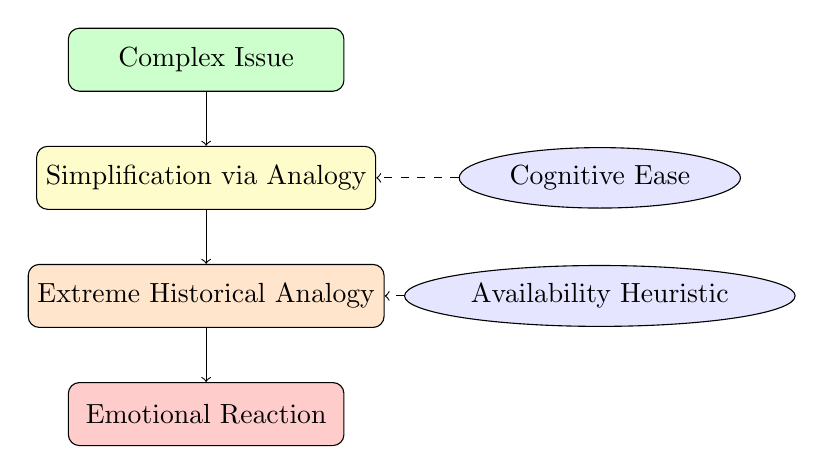
\begin{tikzpicture}
			% Main process boxes
			\node[draw, rectangle, rounded corners, fill=green!20, minimum width=3.5cm, minimum height=0.8cm] (complex) at (0,0) {Complex Issue};
			\node[draw, rectangle, rounded corners, fill=yellow!20, minimum width=3.5cm, minimum height=0.8cm] (simplify) at (0,-1.5) {Simplification via Analogy};
			\node[draw, rectangle, rounded corners, fill=orange!20, minimum width=3.5cm, minimum height=0.8cm] (extremes) at (0,-3) {Extreme Historical Analogy};
			\node[draw, rectangle, rounded corners, fill=red!20, minimum width=3.5cm, minimum height=0.8cm] (emotion) at (0,-4.5) {Emotional Reaction};
			
			% Arrows connecting them
			\draw[->] (complex) -- (simplify);
			\draw[->] (simplify) -- (extremes);
			\draw[->] (extremes) -- (emotion);
			
			% Psychological factors (on the right)
			\node[draw, ellipse, fill=blue!10] (cognitive) at (5,-1.5) {Cognitive Ease};
			\node[draw, ellipse, fill=blue!10] (availability) at (5,-3) {Availability Heuristic};
			
			% Connect psychological factors
			\draw[->, dashed] (cognitive) -- (simplify);
			\draw[->, dashed] (availability) -- (extremes);
		\end{tikzpicture}
	}
	\end{center}
\end{frame}

\begin{frame}{Competing Analogies: How to Weigh Them Against Each Other}
	\begin{itemize}
		\item In many debates, multiple competing analogies are proposed for the same situation or concept.
		\item Evaluating competing analogies requires identifying which one captures the morally or legally relevant features of the case.
		\item The strength of an analogy depends not just on the number of similarities but on whether it highlights the features essential to the normative question.
	\end{itemize}
	
	\begin{block}{Framework for Evaluating Competing Analogies}
		\scriptsize
		\begin{enumerate}
			\item Identify the question or issue the analogies are meant to address.
			\item For each analogy, list the relevant similarities and differences with the target case.
			\item Determine which similarities and differences are most relevant to the underlying question.
			\item Consider whether any proposed analogy might obscure important unique features of the target case.
			\item Evaluate whether empirical evidence supports the assumptions built into each analogy.
		\end{enumerate}
	\end{block}
\end{frame}

\begin{frame}{Cultural Differences in Analogical Reasoning}
	\begin{itemize}
		\item Research suggests that the patterns and prevalence of analogical reasoning vary across cultures.
		\item Some East Asian philosophical traditions emphasize relational analogies and correlative thinking more prominently than Western traditions.
		\item Cultural background influences which analogies seem intuitive or persuasive to different audiences.
		\item Awareness of cultural differences in analogical reasoning is important for cross-cultural ethics and legal discussions.
	\end{itemize}
	
	\begin{block}{Examples of Cultural Variations}
		\scriptsize
		\begin{itemize}
			\item \textbf{Confucian Ethics:} Emphasizes family-based analogies, extending familial relationships to social and political contexts.
			\item \textbf{Buddhist Reasoning:} Often uses analogies of illusion and impermanence drawn from natural phenomena.
			\item \textbf{Western Traditions:} Often emphasizes rule-based analogies and categorical similarities.
			\item \textbf{Indigenous Knowledge Systems:} Frequently employ ecological analogies that highlight interconnections between human and natural worlds.
		\end{itemize}
	\end{block}
\end{frame}

\begin{frame}{Analogies in Political Discourse: Persuasion or Manipulation?}
	\begin{itemize}
		\item Political discourse relies heavily on analogies to frame issues, simplify complex policies, and evoke emotional responses.
		\item Effective political analogies connect abstract policies to concrete experiences that resonate with voters.
		\item The line between persuasive analogical reasoning and manipulative oversimplification is often blurred in political rhetoric.
		\item Critical evaluation of political analogies requires identifying both their legitimate insights and their misleading simplifications.
	\end{itemize}
	
	\begin{table}
		\scriptsize
		\begin{tabular}{|p{2.5cm}|p{4cm}|p{4cm}|}
			\hline
			\textbf{Political Domain} & \textbf{Common Analogies} & \textbf{Rhetorical Function} \\
			\hline
			Economic Policy & Government budget as household budget & Simplify macro concepts \\
			\hline
			Foreign Policy & International relations as schoolyard dynamics & Humanize complex relationships \\
			\hline
			Social Policy & Society as family/team/machine & Frame value priorities \\
			\hline
			Environmental Policy & Earth as patient/home/resource & Frame relationship to nature \\
			\hline
		\end{tabular}
	\end{table}
\end{frame}

\begin{frame}{The Limits of Analogical Reasoning in Complex Systems}
	\begin{itemize}
		\item Analogical reasoning faces significant challenges when applied to highly complex systems with emergent properties.
		\item In domains like climate science, economics, or artificial intelligence, simple analogies often fail to capture crucial system dynamics.
		\item The \textbf{complexity limitation} reflects how analogies necessarily simplify by focusing on specific features while ignoring others.
		\item Awareness of these limits helps prevent overconfidence in conclusions drawn from analogical reasoning about complex systems.
	\end{itemize}
	
	\begin{alertblock}{Warning Signs of Analogy Breakdown}
		\scriptsize
		The usefulness of an analogy may be compromised when:
		\begin{itemize}
			\item The system exhibits emergent properties not present in any of its components
			\item Non-linear relationships dominate the system behavior
			\item Multiple feedback loops create unpredictable dynamics
			\item Scale differences between source and target fundamentally change relevant properties
			\item The system adapts or evolves in response to interventions
		\end{itemize}
	\end{alertblock}
\end{frame}

\begin{frame}{Conclusion: Analogical Reasoning as a Bridge Between Experience and New Territory}
	\scriptsize
	\begin{itemize}
		\item Analogical reasoning serves as a cognitive bridge from familiar experiences to novel situations and abstract concepts.
		\item Strong analogical arguments focus on relevant similarities, account for significant disanalogies, and consider base rates.
		\item In ethics and law, competing analogies often illuminate different aspects of complex issues and embody different normative commitments.
		\item Developing skill in creating and evaluating analogies enhances critical thinking across disciplines and contexts.
	\end{itemize}
	
	\begin{center}
		 \resizebox{0.7\textheight}{!}{%
		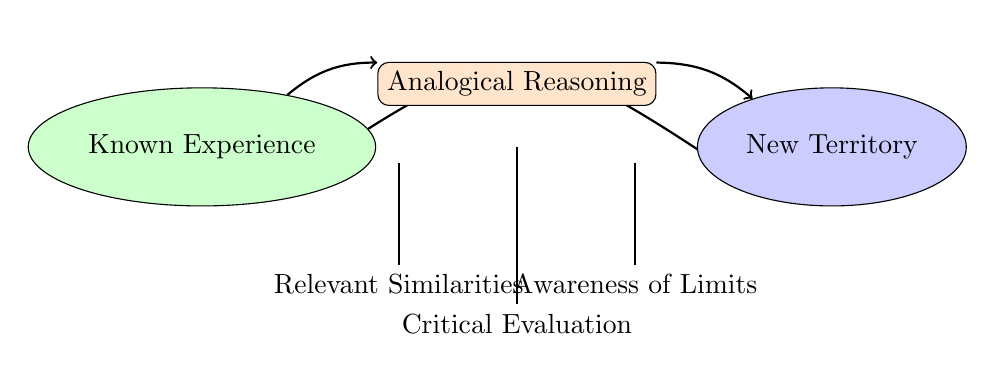
\begin{tikzpicture}
			% Set up the bridge structure
			\draw[thick] (-5,0) -- (-3,0);
			\draw[thick] (3,0) -- (5,0);
			
			% Bridge arch
			\draw[thick] (-3,0) .. controls (0,2) .. (3,0);
			
			% Left side - Known territory
			\node[draw, ellipse, fill=green!20, minimum width=2.5cm, minimum height=1.5cm] (known) at (-4,0.5) {Known Experience};
			
			% Right side - New territory
			\node[draw, ellipse, fill=blue!20, minimum width=2.5cm, minimum height=1.5cm] (new) at (4,0.5) {New Territory};
			
			% Bridge label
			\node[draw, rectangle, rounded corners, fill=orange!20] (bridge) at (0,1.3) {Analogical Reasoning};
			
			% Arrows
			\draw[->, thick] (known) to[bend left=20] (bridge);
			\draw[->, thick] (bridge) to[bend left=20] (new);
			
			% Supporting pillars of strong analogical reasoning
			\draw[thick] (-1.5,-1) -- (-1.5,0.3);
			\node[below] at (-1.5,-1) {Relevant Similarities};
			
			\draw[thick] (0,-1.5) -- (0,0.5);
			\node[below] at (0,-1.5) {Critical Evaluation};
			
			\draw[thick] (1.5,-1) -- (1.5,0.3);
			\node[below] at (1.5,-1) {Awareness of Limits};
		\end{tikzpicture}
	}
	\end{center}
\end{frame}

\end{document}